\section{Discussion \label{sec:discussion}}

\subsection{Complex Crater Collapse} 

The impact in scenarios A and B forms a complex crater for both acoustic fluidisation models (Figure \ref{fig:comparison}). In order for this to happen, wholesale crater collapse must occur. Both models induce enough weakening to achieve this, but the style of weakening differs between the two.

As described in sections \ref{sec:blockvelo} and \ref{sec:meloshvelo}, the spatial characteristics of acoustic energy are different in the two models. In the block model, for scenarios A and B, dissipation of acoustic energy mainly occurs laterally (Figure \ref{fig:block_velo}). The longevity of intense vibrations is thus greatest vertically, inferring that complex crater collapse is induced by a deep weakening, centered mainly under the central uplift. This is reinforced through the subcrater deformation in scenarios A and B; the central uplift in A is very large, and extends deep into the target (Figure \ref{fig:block_deformation}). The lateral extent of vibrations is still enough, however, to produce a wide central uplift. 

The lack of acoustic vibrations at the crater rim during modification in the block model (Figure \ref{fig:block_velo}) suggests that crater rim collapse is not a direct consequence of acoustic vibrations. This may be one of the reasons why the block model fails to produce discrete, terraced fault blocks at the crater rim in numerical simulations of crater collapse \citep{kenkmann2012modification}.

In the Melosh model, rapid vertical decay of vibrations removes intense vibrations from depth  in both scenarios A and B (Figure \ref{fig:melosh_velo}). Yet, crater collapse still occurs, suggesting that collapse is facilitated by shallow acoustic vibrations. Again, this is reinforced by the large, shallow, deformation shown in Figure \ref{fig:melosh_deformation}. Importantly, a large amount of acoustic energy is regenerated in scenarios A and B, particularly under the central uplift and crater rim at shallow depths. Shallow regeneration of acoustic energy in these areas also results in crater collapse for this set of acoustic fluidisation parameters. This is in contrast to the block model, where no regeneration of acoustic energy and deep weakening result in collapse.

\subsection{Crater Morphology}

\begin{table}[!t]
\small
\centering
\begin{tabular*}{\linewidth}{@{\extracolsep{\fill} }p{1.5cm} c c c c}
\toprule
& \multicolumn{4}{c}{Dimension} \\ \cmidrule{2-5}
Crater & $D$ (km) & $d$ (km) & $d/D$ & $d_{s}$ (km) \\ \midrule
Block, A & 113 & 0.948 & 0.0084 & 1.145$^b$\\
Melosh, A & 154 & 0.596 & 0.0039 & 1.308$^b$\\ \midrule
Block, B & 14.8 & 0.345 & 0.0233 & 0.478$^b$\\
Melosh, B & 17.2 & 0.146 & 0.0085 & 0.510$^b$\\ \midrule
Block, C & 2.06 & 0.464 & 0.2256 & 0.407$^a$\\
Melosh, C & 1.97 & 0.474 & 0.2408 & 0.389$^a$\\ 
\bottomrule
\end{tabular*}
\caption{Table of crater dimensions for all scenarios. $D$ = diameter, $d$ = depth, and $d_{s}$ = scaling law depth. Scaling law a; \citet{pike1977apparent}, b; \citet{grieve1992terrestrial}}.\label{tb:crater_dimensions}
\end{table}

Both models produce similar crater morphologies for each scenario, as shown in Figure \ref{fig:comparison}. While the craters formed are of the same type, their depth and diameter differ. Table \ref{tb:crater_dimensions} shows crater depth, $d$, scaling law depth, $d_{s}$, diameter, $D$, and depth-to-diameter ratio for all block and Melosh model scenarios. 

Similar crater dimensions are formed by both models for the simple crater in scenario C. As discussed earlier, the deformation and vibrational velocity field are also very alike in this scenario. At this scale and for this set of parameters, the block and Melosh models produce very similar results.

\begin{figure*}[bp]

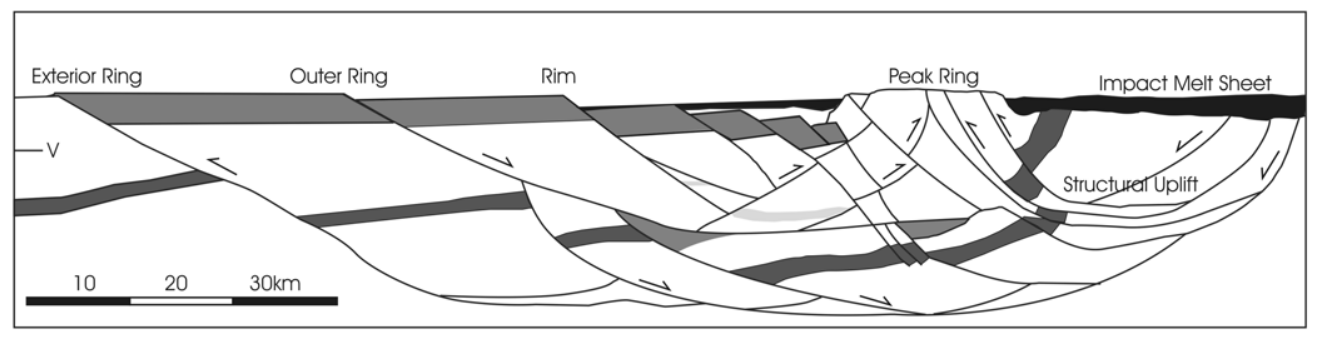
\includegraphics[width=\linewidth]{images/grieve_model.png}
\caption{Structural model of the peak rings at Vredfort, Chicxulub and Sudbury craters from \citet{grieve2008observations}. Here the the peak ring is formed at the confluence of inwardly and outwardly collapsing material. This model is, however, inconsistent with seismic observations at Chicxulub \citep{morgan2011full}, where outer ring material is forced directly under the forming peak ring.}\label{fig:grieve_model}
\end{figure*}

The depth and diameter scaling law for simple craters used in Table \ref{tb:crater_dimensions} \citep{pike1977apparent}:

\vspace{-0.2cm}
\begin{equation}\label{eq:simple_scaling}
d=0.196 D^{1.01},
\end{equation}

yields similar crater depths for both models in scenario C. The model depths are very similar to those predicted by the scaling law, although the block model is a closer approximation.

In scenario A similar crater dimensions are formed in both models, but as is obvious from Figure \ref{fig:comparison}, the crater diameter is considerably larger in the Melosh model and the depth is smaller. Overall, this results in a depth-to-diameter ratio that is smaller than the block model, but still the same order of magnitude.

The greatest difference in crater morphology, both quantitatively and qualitatively, is in scenario B. This is evident from both Table \ref{tb:crater_dimensions} and Figure \ref{fig:comparison}. The depth-to-diameter ratio differs by an order of magnitude between the two models. The Melosh model takes the smaller value, similar to the depth-to-diameter ratios recorded in scenario A.

A scaling law developed by \citet{grieve1992terrestrial} for complex craters in crystalline targets:

\vspace{-0.2cm}
\begin{equation}\label{eq:complex_scaling}
d=0.15 D^{0.43},
\end{equation}

is compared to the block and Melosh models for scenario B. The recorded block model depth is approximately 100m shallower than that predicted by the scaling law, whereas the Melosh model is around 300m shallower. Again, the block model produces the better approximation.

The scaling laws applied here are not perfect. They are based on terrestrial crater data, which is, due to erosion, poor at best. For simple craters, the two models agree very well with the scaling laws, each producing craters around 400m deep. The block model depths for complex craters are also reasonably close, differing by 100-200m from the scaling law. However, the Melosh model produces complex craters that are up to 700m shallower than that predicted by the scaling law. Thus, for this set of parameters, the Melosh model consistently underestimates complex crater depth while the block model produces a close approximation. This is perhaps unsurprising given how little the Melosh model has been tested when compared to the block model.

\subsection{Peak Ring Formation}

Both the block and Melosh models for scenario A form a peak ring. However, there is some debate as to quite how peak rings form in complex craters, as observational evidence has lead to conflicting mechanisms. 

The block model results presented here are similar to hydrocode simulations performed by \citet{collins2002hydrocode} and \citet{ivanov2005numerical}. Simulations of Chicxulub crater formation indicate that the inwardly collapsing crater rim is forced underneath the outwardly collapsing central uplift, forming the inner peak ring \citep{collins2002hydrocode}. These results agree well with seismic observations of the peak ring and its internal structure at Chicxulub \citep{morgan2011full}. Inward dipping reflectors are interpreted from the seismic data, indicating that inwardly collapsing crater material is indeed forced underneath the forming peak ring. The block model velocity field shown in Figure \ref{fig:peak_ring} supports this observation, reinforcing an already well known mechanism for peak ring formation.

\citet{grieve2008observations} observed structural evidence for an alternative mechanism of peak ring formation at Vredfort crater, South Africa (Figure \ref{fig:grieve_model}). The 120-200km diameter impact crater \citep{turtle2005impact} is one of the biggest on Earth, and has the morphology of a complex, peak ring impact crater. The structural model of a terrestrial ring basin produced by \citet{grieve2008observations}, shown in Figure \ref{fig:grieve_model}, is one which suggests that the peak ring is a result of uplift at the confluence of inwardly and outwardly collapsing crater material. The velocity field during peak ring formation for the Melosh model in scenario A (Figure \ref{fig:peak_ring}) suggests that this mechanism may well be a viable one. This also enhances the credibility of the Melosh model presented here.

The relative timing of when material outside and inside the peak ring begin to collapse may be key in deciding which of the two mechanisms comes into play during peak ring formation \citep{grieve2008observations}. Certainly, the observations from Chicxulub and Vredfort discussed above suggest that either mechanism may be relevant for peak ring formation. As the block model favours observations from Chicxulub, while the Melosh model favours observations from Vredfort, it is difficult to say which model produces the 'better' approximation. Clearly, a study of Chicxulub and Vredfort crater formation using both the block and Melosh models would be useful. 


\subsection{Melosh Model Parameter Space and Sensitivity}

To sufficiently weaken the target rock for any length of time, it was found that  $\lambda$ could be as high as $0.2a$. As $\lambda$ decreases with impactor radius, the rate of dissipation increases, as described in section \ref{sec:parameters}. This results in faster acoustic energy dissipation for smaller impacts. However, making $\lambda$ too small ($0.05a$) resulted in complex craters being formed in scenarios A, B and C, which is unrealistic for terrestrial impacts. This is because the effective viscosity, $\eta_{\text{eff}}$, is proportional to $\lambda$ (equation \ref{eq:yield_vib}).

There exists a trade-off between the longevity of vibrations, governed by $\lambda Q$, and the magnitude of weakening, governed primarily by $\lambda$. A comprehensive study of $\lambda$ and $\lambda Q$ parameter space would be useful in determining how variations in these two parameters influence crater morphology and subcrater deformation. Realistically, the value of $Q=10$ used here is at least an order of magnitude too small \citep{melosh1996dynamical,anderson1989theory}. However, the product $\lambda Q$, where $Q=10$ and $\lambda = 0.2a$, is small enough that complex craters are formed in scenarios A and B, and not in C (Figure \ref{fig:comparison}). If $\lambda Q$ is an order of magnitude bigger, the dissipation term becomes so small that, again, complex craters are created in all three scenarios as vibrations do not dissipate fast enough.

To increase $Q$ by an order of magnitude, $\lambda$ must decrease by an order of magnitude (i.e., $0.01$-$0.02a$). This is not possible with the current model, as $\lambda$ would become smaller than the cell size and thus spatial variations in acoustic energy would not be fully resolved. As such, this is a problem regarding resolution. By increasing the resolution these changes to $\lambda$ and $Q$ could be tested. Given the non-linearity of the Melosh model, however, it is hard to say if these parameter changes will result in the predicted crater morphologies for all three scenarios. Clearly, this is an area for further study.